\documentclass[11pt, oneside]{article}   	% use "amsart" instead of "article" for AMSLaTeX format


\usepackage{draftwatermark}
\SetWatermarkText{Draft}
\SetWatermarkScale{6}
\SetWatermarkLightness {0.80} 
% \SetWatermarkColor[rgb]{0.7,0,0}


\usepackage{geometry}                		% See geometry.pdf to learn the layout options. There are lots.
\geometry{letterpaper}                   		% ... or a4paper or a5paper or ... 
%\geometry{landscape}                		% Activate for for rotated page geometry
%\usepackage[parfill]{parskip}    		% Activate to begin paragraphs with an empty line rather than an indent
\usepackage{graphicx}				% Use pdf, png, jpg, or eps� with pdflatex; use eps in DVI mode
								% TeX will automatically convert eps --> pdf in pdflatex		
\usepackage{amssymb}
\usepackage{hyperref}
\usepackage{url}
\usepackage{authblk}
\usepackage{amsmath}
\usepackage{graphicx}
\usepackage{fixltx2e}
\usepackage{hyperref}
\usepackage{alltt}
\usepackage{color}

\usepackage{authblk}



\title{Automating the Discovery of Features in Network Datasets using Deep Learning: A Proposed Collaboration Between Brocade and RSA Security LLC.}


\author[1] {David Meyer, Hadi Nahari, and Mark Presti}
\affil[1] {\{dmm,hnahari,mpresti\}@brocade.com}

% \date{}							% Activate to display a given date or no date


\begin{document}
\maketitle
\begin{abstract}
Recent advances in machine learning, coupled with the onslaught of data being collected from a wide variety of sensors has rekindled interest in using machine learning as a method to uncover hidden structure in these ever growing data sets. In particular, advances in the design of multi-layer deep artificial neural networks (DNNs) combined with effective approaches for training DNNs has opened up the opportunity to use DNNs for novel applications ranging from speech recognition and generation to self-driving vehicles. DNNs are  multiple-layer architectures (deep architectures) which extract inherent features in data and  discover important hidden structure in diverse data sets. Given that the factors contributing to traffic flow, congestion, and queuing delay in a data center result from the non-obvious interaction of complex factors, DNNs represent a novel and powerful method for learning how these factors interact and for predicting a wide variety of complex network behaviors. These same DNNs can be used to detect various Advanced Persistent Threats in the security domain. This document introduces a specific form of DNN, and provides a framework for an ongoing joint project between Brocade and RSA Security LLC. The work is intended to be carried out using the datasets acquired from the Massachusetts Open Cloud (MOC).
\end{abstract}

\section{Introduction} 

Recent advances in machine learning, coupled with the onslaught of data being collected from a wide variety of sensors has rekindled interest in using machine learning as a method to uncover hidden structure in these ever growing data sets\footnote{This  phenomena is evidenced by the explosive growth in the number of "data analytics" startups~\cite{ANALYTICS}.}. In particular, advances in the design of multi-layer deep artificial neural networks (DNNs) combined with effective approaches for training DNNs has opened up the opportunity to use DNNs for novel applications ranging from speech recognition and generation to self-driving vehicles. DNNs are  multiple-layer architectures (deep architectures) which extract inherent features in data and  discover important hidden structure in diverse data sets. Given that the factors contributing to traffic flow, congestion, and queuing delay in a data center result from the non-obvious interaction of complex factors, DNNs represent a novel and powerful method for learning how these factors interact and for predicting a wide variety of complex network behaviors. A key research question however is how to find the key features that explain the variation in the datasets that we observe. Automating such \emph{feature discovery} is one of the primary goals of this research. The second important goal proposed here is the generation and publication of standardized network datasets for use by researchers and industrial partners.\footnote{See ImageNet \cite{ImageNet} as an example of a standardized dataset for machine learning practitioners and researchers.}

Neural networks had traditionally been trained with an algorithm called back propagation~\cite{WIDROW2002}, which is so named because the algorithm propagates the error in the neural network's estimate \emph{backward} from the output layer towards the input layer. Back propagation also requires labeled data sets; these \emph{training} sets have elements of the form $(\mathbf{x}^{(i)},\mathbf{t}^{(i)})$, where the $\mathbf{x}^{(i)}$ are the inputs and the $\mathbf{t}^{(i)}$ are the targets (the targets tell what the data is, for example, "cat"). The DNN computes an output value, sometimes called (largely for historical reasons) the hypothesis  $h_\theta(\mathbf{x}^{(i)})$.  $h_\theta(\mathbf{x}^{(i)})$  is then compared to the target $\mathbf{t}^{(i)}$ and the difference $h_\theta(\mathbf{x}^{(i)}) - \mathbf{t}^{(i)}$  is taken as an estimate of the model's error. This error is then "back propagated" (with the help of additional algorithmic machinery) down the DNN from output to input, adjusting the model parameters along the way. Back propagation is an instance of a  \emph{supervised learning} algorithm since it requires labeled data. Training algorithms that use unlabeled data are referred to as \emph{unsupervised learning} algorithms.

There were, however, several weaknesses with the back propagation algorithm which essentially limited the utility of DNNs. These included the fact that back propagation really didn't work well in deep networks (for technical reasons relating to the computation of what are called gradients) and the tendency for the algorithm to fall into poor local minima when the DNN was initialized with random weights\footnote{The problem of non-optimal minima is a property of non-convex optimization, where local minima aren't necessarily global minima when the some of the DNNs parameters were initialized with random values~\cite{CHIANG2011}.}. The requirement for labeled data sets was also a problem since most data is unlabeled.  These two problems with DNNs,  the need for labeled training sets and ineffective training via back propagation, were largely overcome by the groundbreaking work of Geoffrey Hinton and his colleagues in 2006~\cite{HINTON2006}. Hinton's breakthrough was to show that unsupervised, greedy, layerwise training of DNNs was effective in overcoming the problems with traditional back propagation training. This is discussed in more detail in Section~\ref{sec:sae}.

\section{So What Is An  AutoEncoder?} 
\label{sec:auto-encoder}
In this section we introduce our basic methodology which is based on a deep-learning based prediction model. A stacked \emph{autoencoder}~\cite{BENGIO2007} model is used to learn generic features, and as such is part of a \textit{representation learning} system. In this proposal we intend to exploit techniques such as unsupervised deep learning (e.g., via autoencoders) to automatically learn network features of interest.  As such this section reviews basic autoencoder and stacked autoencoder technology. 

\subsection{The Basic Autoencoder}
\label{sec:basic}
The traditional autoencoder is an artificial neural network that attempts to reproduce its input, i.e., the target output is the input.  More formally (and following the notation of~\cite{VINCENT2008}), an autoencoder takes an input vector $\mathbf{x} \in [0,1]^d$ and maps it to a hidden representation $\mathbf{y} \in [0,1]^d$ through a deterministic mapping $\mathbf{y} = f_{\theta}(\mathbf{x}) = s(\mathbf{Wx} + b)$, parameterized by $\theta = \{\mathbf{W,b}\}$. $\mathbf{W}$ is a $d^\prime \times d$ weight matrix, $\mathbf{b}$ is a bias vector and $s$ is the \emph{sigmoid}\footnote{Note that the sigmoid activation function $s$ "squashes" its input into the range $[0,1]$} activation function, $s(\mathbf{x}) = \frac{1}{1 + e^{-\mathbf{x}}}$. The hidden representation $\mathbf{y}$, sometimes called the \emph{latent} representation,  is then mapped back to a �reconstructed� vector $\mathbf{z} \in [0,1]^d$, where  $\mathbf{z} = g_{\theta\prime}(\mathbf{y}) = s(\mathbf{W}^\prime\mathbf{y} + \mathbf{b}^\prime)$, with $\theta^\prime = \{\mathbf{W}^\prime, \mathbf{b}^\prime\}$. This scenario is depicted in cartoon form in Figure~\ref{fig:autoencoder}. Thus each training $\mathbf{x}^{(i)}$ is thus mapped to a corresponding $\mathbf{y}^{(i)}$ and a reconstruction (of $\mathbf{x}^{(i)}$) $\mathbf{z}^{(i)}$.  Finally, note that  the weight matrix $\mathbf{W}^\prime$ may optionally be constrained by $\mathbf{W}= \mathbf{W}^{T}$, in which case the autoencoder is said to have \emph{tied} weights. Each training example $\mathbf{x}^{(i)}$ is thus mapped to a corresponding $\mathbf{y}^{(i)}$ which is then mapped to a reconstruction $\mathbf{z}^{(i)}$ such that $\mathbf{z}^{(i)} \approx \mathbf{x}^{(i)}$.  

The basic idea here is that the autoencoder is constructed in such a way that the mapping $\mathbf{x}^{(i)} \mapsto \mathbf{y}^{(i)}$ reveals essential structure in the input vector $\mathbf{x}^{(i)}$ that is not otherwise obvious. For example, if the autoencoder has fewer hidden units than input units it must find a representation that essentially compresses the input in such a way that it can be efficiently reconstructed. The compressed representation has lower dimensionality than the input and is represents an \emph{abstraction} of the input. In the case of image recognition  $\mathbf{x}^{(i)}$ might be an image (pixels) while $\mathbf{y}^{(i)}$ might consist of edges in various orientations.

\begin{figure}
\center{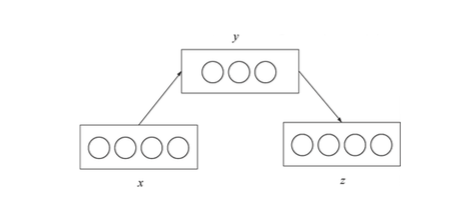
\includegraphics{images/autoencoder.png}}
\caption{Classic Autoencoder}
\label{fig:autoencoder}
\end{figure}


The parameters $\theta$ and $\theta^{\prime}$ of the model are optimized to minimize the \emph{average reconstruction error} as shown in Equation~\ref{eqn:loss}:

\begin{equation}
\begin{split}
\theta^{*}, \theta^{\prime *} = \operatorname*{arg\,min}_{\theta,\theta^\prime} \frac{1}{n}\sum\limits_{i = 1}^{n}L\left(\bold{x}^{(i)},\bold{z}^{(i)}\right) \\
 = \operatorname*{arg\,min}_{\theta, \theta^{\prime}} \frac{1}{n}\sum\limits_{i = 1}^{n}L\left(\mathbf{x}^{(i)}, g_{\theta^\prime}(f_\theta(\mathbf{x}^{(i)})\right)
\end{split}
\label{eqn:loss}
\end{equation}


Here $L$ is a loss function such as the traditional squared error $L(\mathbf{x}, \mathbf{z}) =   \parallel \mathbf{x} -  \mathbf{z}\parallel^{2}_{2}$. Note that if  $\mathbf{x}$ and $\mathbf{z}$ can be interpreted as either bit vectors or vectors or probabilities (i.e., they are Bernoulli probability vectors), then the \emph{reconstruction cross-entropy}, as defined in Equation~\ref{eqn:cross-entropy}, can be used.

\begin{equation}
\begin{split}
L_{\mathcal{H}}(\mathbf{x},\mathbf{z}) = \mathcal{H}(\mathcal{B}_\mathbf{x},\mathcal{B}_\mathbf{z}) \\
= - \sum\limits_{k = 1}^{d}[\mathbf{x}_k \log \mathbf{z}_k + (1 - \mathbf{x}_k) \log (1 - \mathbf{z}_k)]
\end{split}
\label{eqn:cross-entropy}
\end{equation}

More generally, this methodology casts learning as \emph{optimization} using Empirical Risk Minimization~\cite{BENGIO2013}. The Empirical Risk $\hat{R}$ is defined as
\begin{equation}
\hat{R}(f_\theta,D_n) = \sum\limits_{i = 1}^{n}L\left(f_\theta(\mathbf{x}^{(i)}), \mathbf{z}^{(i)}\right)
\label{en:empirical-risk}
\end{equation}
In some cases it may be necessary to induce a preference for some values of the parameters to avoid �overfitting�~\cite{DIETTERICH95}. To avoid overfitting we can define a \emph{Regularized Empirical Risk}, where the regularization imposes a degree of sparseness on the derived encodings. Suppose we have a training set 
$D_n = \{\mathbf{x}^{(1)},\mathbf{x}^{(2)},...,\mathbf{x}^{(n)}\}$. Then the \emph{Regularized Empirical Risk} is defined as follows:
\begin{equation}
\hat{R}_\lambda(f_\lambda,D_n) = \left( \sum\limits_{i = 1}^{D_n}L\left(f_\theta(\mathbf{x}^{(i)}), \mathbf{z}^{(i)}\right)\right) + \lambda\Omega(\theta)
\end{equation}
where $\Omega$ penalizes more or less certain parameter values and $\lambda \geq 0$ controls the amount of regularization. Regularizers generally perform two basic functions: First, a regularizer can keep the autoencoder from learning the identity function (in which case the autoencoder would be useless).  The second function that a regularizer provides is that it enforces certain properties on the weights. For example, using the  L1-norm\footnote{The L1-norm is sometimes called the \textit{taxicab} norm} as a regularizer, where the L1-norm $ \parallel \mathbf{x}\parallel_{1}  = \sum\limits_{i}^{n}\mid x_{i} \mid$, enforces spareness on the vector $\boldsymbol x $. This is because in order to minimize  $\parallel \mathbf{x}\parallel_{1}$, some (or most) of the $x_i$ have to be zero.  On the other hand, using the L2-norm\footnote{The L2-norm is sometimes called the \textit{Euclidean} norm} is defined as follows: Let $\mathbf{x}$ be an n-dimensional vector in $\mathbb{R}^n$. Then the L2-norm $\parallel \mathbf{x} \parallel_{2}  = \left(\sum\limits_{i = 1}^{n}\mid x_{i} \mid^2\right)^{\frac{1}{2}}$, which forces the $x_i$ (i.e., the weights) to be small \footnote{In general, the p-norm is defined to be $\parallel \mathbf{x} \parallel_{p}  = \left(\sum\limits_{i = 1}^{n}\mid x_{i} \mid^p\right)^{\frac{1}{p}}$.}.

Thus \emph{learning} in this setting amounts to finding optimal parameters $\theta^{*}$ that satisfy $\theta^{*} =\operatorname*{arg\,min}_{\theta}\hat{R}(f_\theta,D_n)$. However, one of the risks of using autoencoders, as mentioned above, is that the autoencoder can potentially learn the identity function and thereby not extract useful features from the input.  This problem is especially acute if the size of the hidden layer has the same number of units as the input layer (or more).  One way to train an autoencoders that has more hidden units than input units to learn useful features is to impose sparsity constraints such as the regularizations described above on the minimization problem~\cite{PALM2012} described in Equation~\ref{eqn:loss}.  The effect is to force the representations found by the hidden layers to be sparse.  Such an autoencoder is referred to as a \emph{sparse autoencoder}. A popular 
 sparsity constraint  is based on the Kullback-Leibler divergence~\cite{CRUZ2011}. The Kullback-Leibler Divergence $\mathcal{D}_{KL}(P\parallel Q)$ can be thought of as a measure of the information lost when probability distribution $Q$ is used to approximate $P$. For our purposes we define $\mathcal{D}_{KL}(\rho\parallel\hat{\rho})$ as follows
 \begin{equation}
\mathcal{D}_{KL}(\rho\parallel\hat{\rho}) = \rho \log\frac{\rho}{\hat{\rho_{j}}} + (1 - \rho) \log \frac{1 - \rho}{1 - \hat{\rho_{j}}}
\label{eqn:kl}
\end{equation}
where $\rho$ is a sparsity parameter who's value is close to zero and $\hat{\rho}_j = \frac{1}{n}\sum\limits_{i = 1}^{n}s(\mathbf{W}\mathbf{x}^{(i)}_{j} + \mathbf{b})$, the average activation of hidden unit $j$. Putting this together with Equation~\ref{eqn:loss} we get the following optimization problem:
\begin{equation}
\operatorname*{arg\,min}_{\theta, \theta^{\prime}} \frac{1}{n}\sum\limits_{i = 1}^{n}L\left(\mathbf{x}^{(i)}, g_{\theta^\prime}(f_\theta(\mathbf{x}^{(i)})\right) +  \gamma\sum\limits_{j = 1}^{H_{D}}\mathcal{D}_{KL}(\rho\parallel\hat{\rho})
\label{eqn:sparse}
\end{equation}
where $H_{D}$ is th number of hidden units and $\gamma$ is a sparsity weighting term. Kullback-Leibler Divergence has the nice property that $\mathcal{D}_{KL}(\rho\parallel\hat{\rho}) = 0$ if $\rho = \hat{\rho}$ (and so weighting these cases improves the sparsity of the encoding; this is the job of the $\gamma$ parameter). 


\subsection{Stacked Autoencoders}
\label{sec:sae}
Stacked Autoencoders (SAEs) are, as the name implies, a stack of single-level autoencoders; hence the SAE  is a deep learning model~\cite{BENGIO2012}. SAEs use the autoencoders described above as building blocks to create a deep network \cite{BENGIO2007}.  While deep architectures can be more expressive and can extract more sophisticated features from input data, until relatively recently deep networks were thought to be too difficult to train and as such of limited utility. As mentioned above, the breakthrough came when Geoffrey Hinton and his colleagues showed how fast, layerwise greedy and unsupervised algorithms can be used to initialize a slower algorithm that fine tunes the learned weights and provides very good results on deep networks~\cite{HINTON2006}. This result revitalized the machine learning community and deep architectures been successfully applied to a wide variety of classification and prediction problems~\cite{DLNET}.


\begin{figure}[ht]
\center{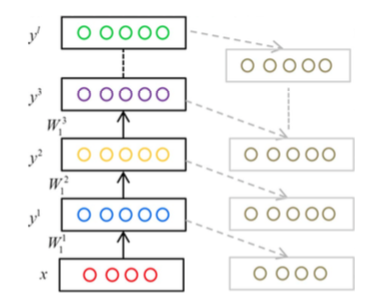
\includegraphics{images/sae_training.png}}
\caption{Layerwise training of a Stacked Autoencoder}
\label{fig:layerwise-training}
\end{figure}


The basic idea behind layerwise training is shown in Figure~\ref{fig:layerwise-training}. The idea  here is to train each layer as described in Equation~\ref{eqn:sparse}. After a layer is trained, the autoencoder output layer is discarded and the features (the $\mathbf{y}^{(i)}$) are used as the input to the next layer. Hence the training is greedy and layerwise. Finally, the last layer in the network, usually either a linear regression layer (if the output values are continuous) or logistic regression layer (if the output is discrete). The final step is to fine tune the network in a supervised fashion using the back propagation algorithm~\cite{WIDROW2002}. The key idea here is that this approach can be used to \emph{automatically} learn the important features in network datasets such as might be collected with Netflow or IPFIX.


\section{Proposed Collaboration}
 \label{sec:collaboration}
 
 The proposed collaboration here is to build an anomaly detection system\footnote{"Anomaly" here is being used in the most general way, i.e., anomaly detection as a classification problem.  Anomalies can be, among other things,  deviations from normal traffic patterns, routing updates, configurations, etc.} based on the workflow shown in 
 Figure \ref{fig:workflow}. As showing in the figure, such a system is comprised of a data collection/ingestion phase, an extract, transform and load (ETL) phases, a model development and evaluation phase, followed by feedback from both evaluation by both technical analysts and the target customer.
 
\hfill \break
\hfill \break
 \begin{figure}[ht]
 \center{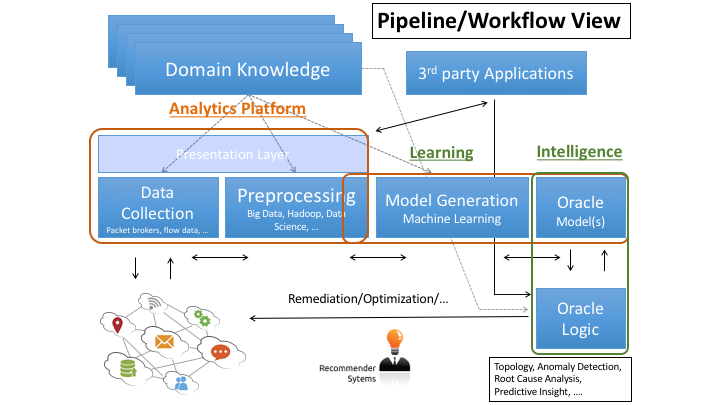
\includegraphics[scale=0.5]{images/workflow.png}}
\caption{Machine Learning Workflow for Network Environments}
\label{fig:workflow}
\end{figure}

\hfill \break
\hfill \break

One of the novel aspects of the proposed work is the idea of using DNNs to automatically detect features of interest in network data and the understanding of such features for use in classification systems such as described above. Of course, there are many other "open" issues in the construction of such a system, such as how to make the system "on-line" so that incremental training is possible within reasonable computational bounds.


 
\section{Milestones and Deliverables}
 \label{sec:milestones}
 \begin{itemize}
 \item M1: Meet with RSA and MOC representatives to review and finalize the proposal
 \item M2: Build data collection infrastructure
 \item M3: Work with RSA data scientists to develop new models for network data
  \item M4: Deploy new models on targeted MOC network segments
 \item M5: Feedback and refinement
 \end{itemize}
 


\section{Acknowledgements}

\newpage
% \cite{test}
\bibliographystyle{plain}
\bibliography{/Users/dmm/papers/bib/ml}
% \bibliography{/Users/dmm/papers/bib/rfc}


\end{document}  


% \begin{equation}
% KL(\rho\parallel\hat{\rho}) = \rho \log\frac{\rho}{\hat{\rho_{j}}} + (1 - \rho) \log \frac{1 - \rho}{1 - \hat{\rho_{j}}}
% \label{eqn:KL}
% \end{equation}

% \begin{equation}
% \begin{array}{cc}\text{minimize} \\ {W_{1}, W_{2}}\end{array}
% \sum\limits_{i = 1}^{m}
% (\parallel {W_{2}W_{1}^{T}x^{(i)} - x^{(i)}}\parallel_{2}^{2}
% + \lambda\sum\limits_{j = 1}^{k}\sqrt{\epsilon + H_{j}(W_{1}^{T}x^{(i)})^{2}})
% \label{eqn:google}
% \end{equation}
